\section{Erreichte Werte}
\subsection{Auswirkung der Größe}
Durch den Aufbau, muss das Verfahren zuverlässig bezüglich der Größe sein, zur Messung wurde der Datensatz von Labeled Faces in the Wild \cite{database_Face} verwendet. In diesem Datensatz ergibt sich im Originalbild eine durchschnittliche Kopfbreite von 94 Pixel.\\
Zur Durchführung wurden die Größe der Bilder mit dem Faktor multipliziert um so kleinere Gesichter zu erhalten und anschließend mit dem Image-Detector von OpenFace zu detektieren, siehe \autoref{img_lineareverkleinerung}.\\
\begin{figure}
	\centering
	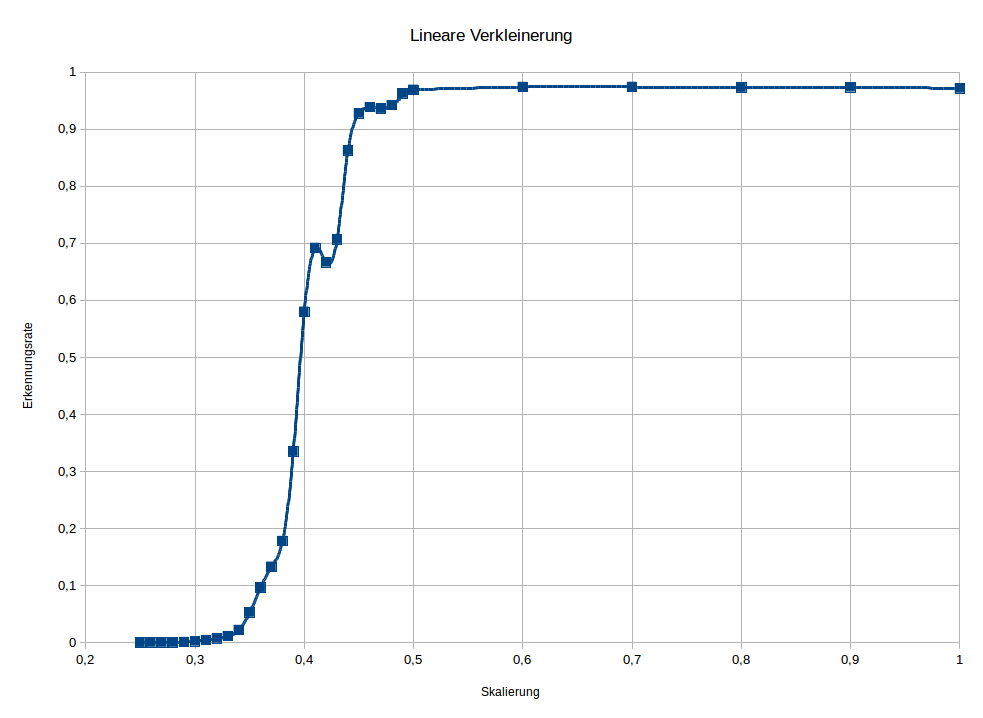
\includegraphics[width=0.5\linewidth]{img/lineare_Verkleinerung}
	\caption{Die Bilder aus Labeled Faces in the Wild \cite{database_Face} wurden mit den Faktor auf der X-Achse linear verkleinert und die Erkennungsrate Y-Achse abgebildet}
	\label{img_lineareverkleinerung}
\end{figure}
Es ist zu erkennen, dass die Wahrscheinlichkeit auf eine erfolgreiche Detektion ab $0.5$, also etwa Gesichert mit 47 Pixel Breite, rapide abnimmt. Bei der verwendeten Kamera \autoref{hardware} entspricht dies einer Distanz von etwa $4.5m$.\\
Bei der maximalen Distanz auf der gearbeitet werden soll $(8.5m)$ ergibt sich eine Gesichtsgröße von etwa 22 Pixel, das einer Skalierung von 0.25 entspricht. Bei dieser Bildgröße ist keine Detektion möglich, siehe \autoref{img_lineareverkleinerung}.
\subsection{verschiedenen Skalierungesverfahren}
Um auf den gewünschten Distanzen arbeiten zu können, wird der jeweilige Bereich Hochskaliert. Dazu wird das Ursprüngliche Bild $(250\times 250)$ linear um den angegebene Faktor verkleinert und anschließend mit den angegebenen Verfahren auf $300\times 300$ wieder vergrößert. Die Wahrscheinlichkeit auf eine Detektion ist in \autoref{img_hochskalliern} abgebildet.\\
\begin{figure}
	\centering
	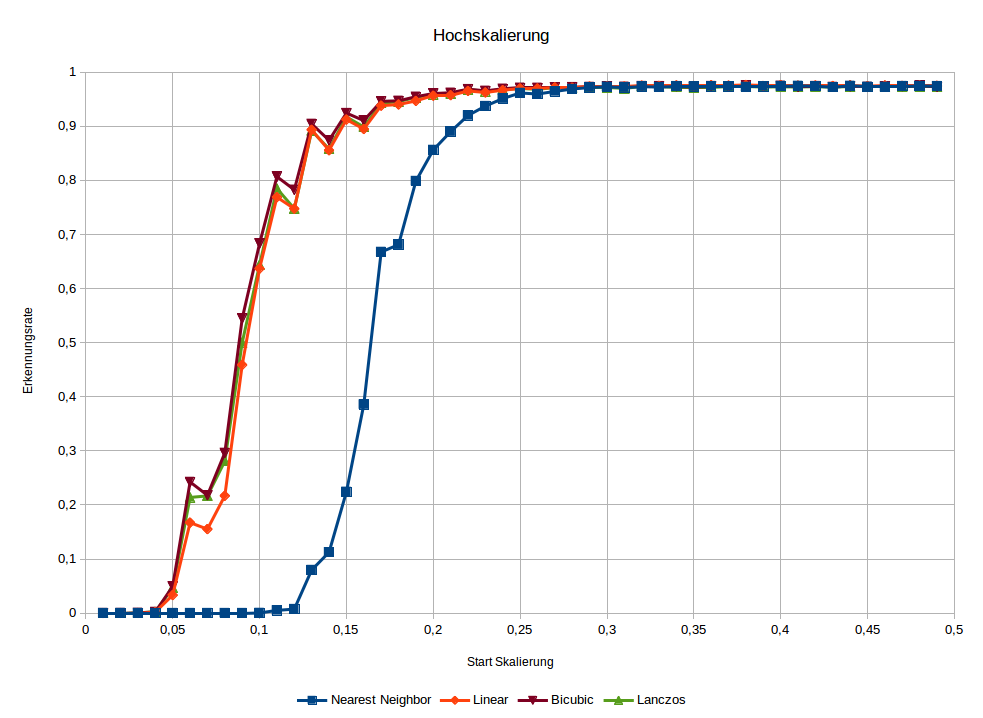
\includegraphics[width=0.5\linewidth]{img/Hochskalliern}
	\caption{Die Bilder aus Labeled Faces in the Wild \cite{database_Face} wurden mit den Faktor auf der X-Achse linear verkleinert und mit den verschiedenen Verfahren wieder vergrößert \autoref{scale_Algos}. Aufgetragen gegen die Detektionswahrscheinlichkeit.
	Nearest-Neighbor (blau), Linear (rot), Bicubic (braun), Lanczos (grün)}
	\label{img_hochskalliern}
\end{figure}
Es ist zu erkennen das durch die Vergrößerung, Gesichter in Bereichen die normal nicht erkennbar sind, bestimmbar werden. Als das ungeeignetste Verfahren hat sich Nearest-Neighbor herausgestellt, siehe blaue Linie \autoref{img_hochskalliern}. Die anderen haben sehr ähnliche Ergebnisse, nur das Lineare Verfahren ist etwas schlechter. Dennoch werden die Anforderungen, einer Detektion auf Gesichtern von 22 Pixel (Skalierung 0.25) von allen erfüllt.\\
Ausgehend vom Skalierungsfaktor des Linearen-, Bicubic- und Lanczos-Verfahren wären mit der verwendeten Kamera auch Distanzen bis zu $14m$ möglich. Allerdings ist das Bild durch die Verkeilung  deutlich besser als Originalaufnahmen, da Pixelrauschen nicht vorhanden ist.
\subsection{Auswirkung von Pixelrauschen}
Durch Aufnahme eines Schwarzbildes der Actioncam zeigt sich, dass das Pixelrauschen recht hoch ist, siehe \autoref{img_noishight}. Das Rauschen hat keine Normalverteilung, sondern es besteht aus kleinen Bereiche, die den selben fehlerhaften Farbwert besitzen.
\begin{figure}
	\centering
	\fbox{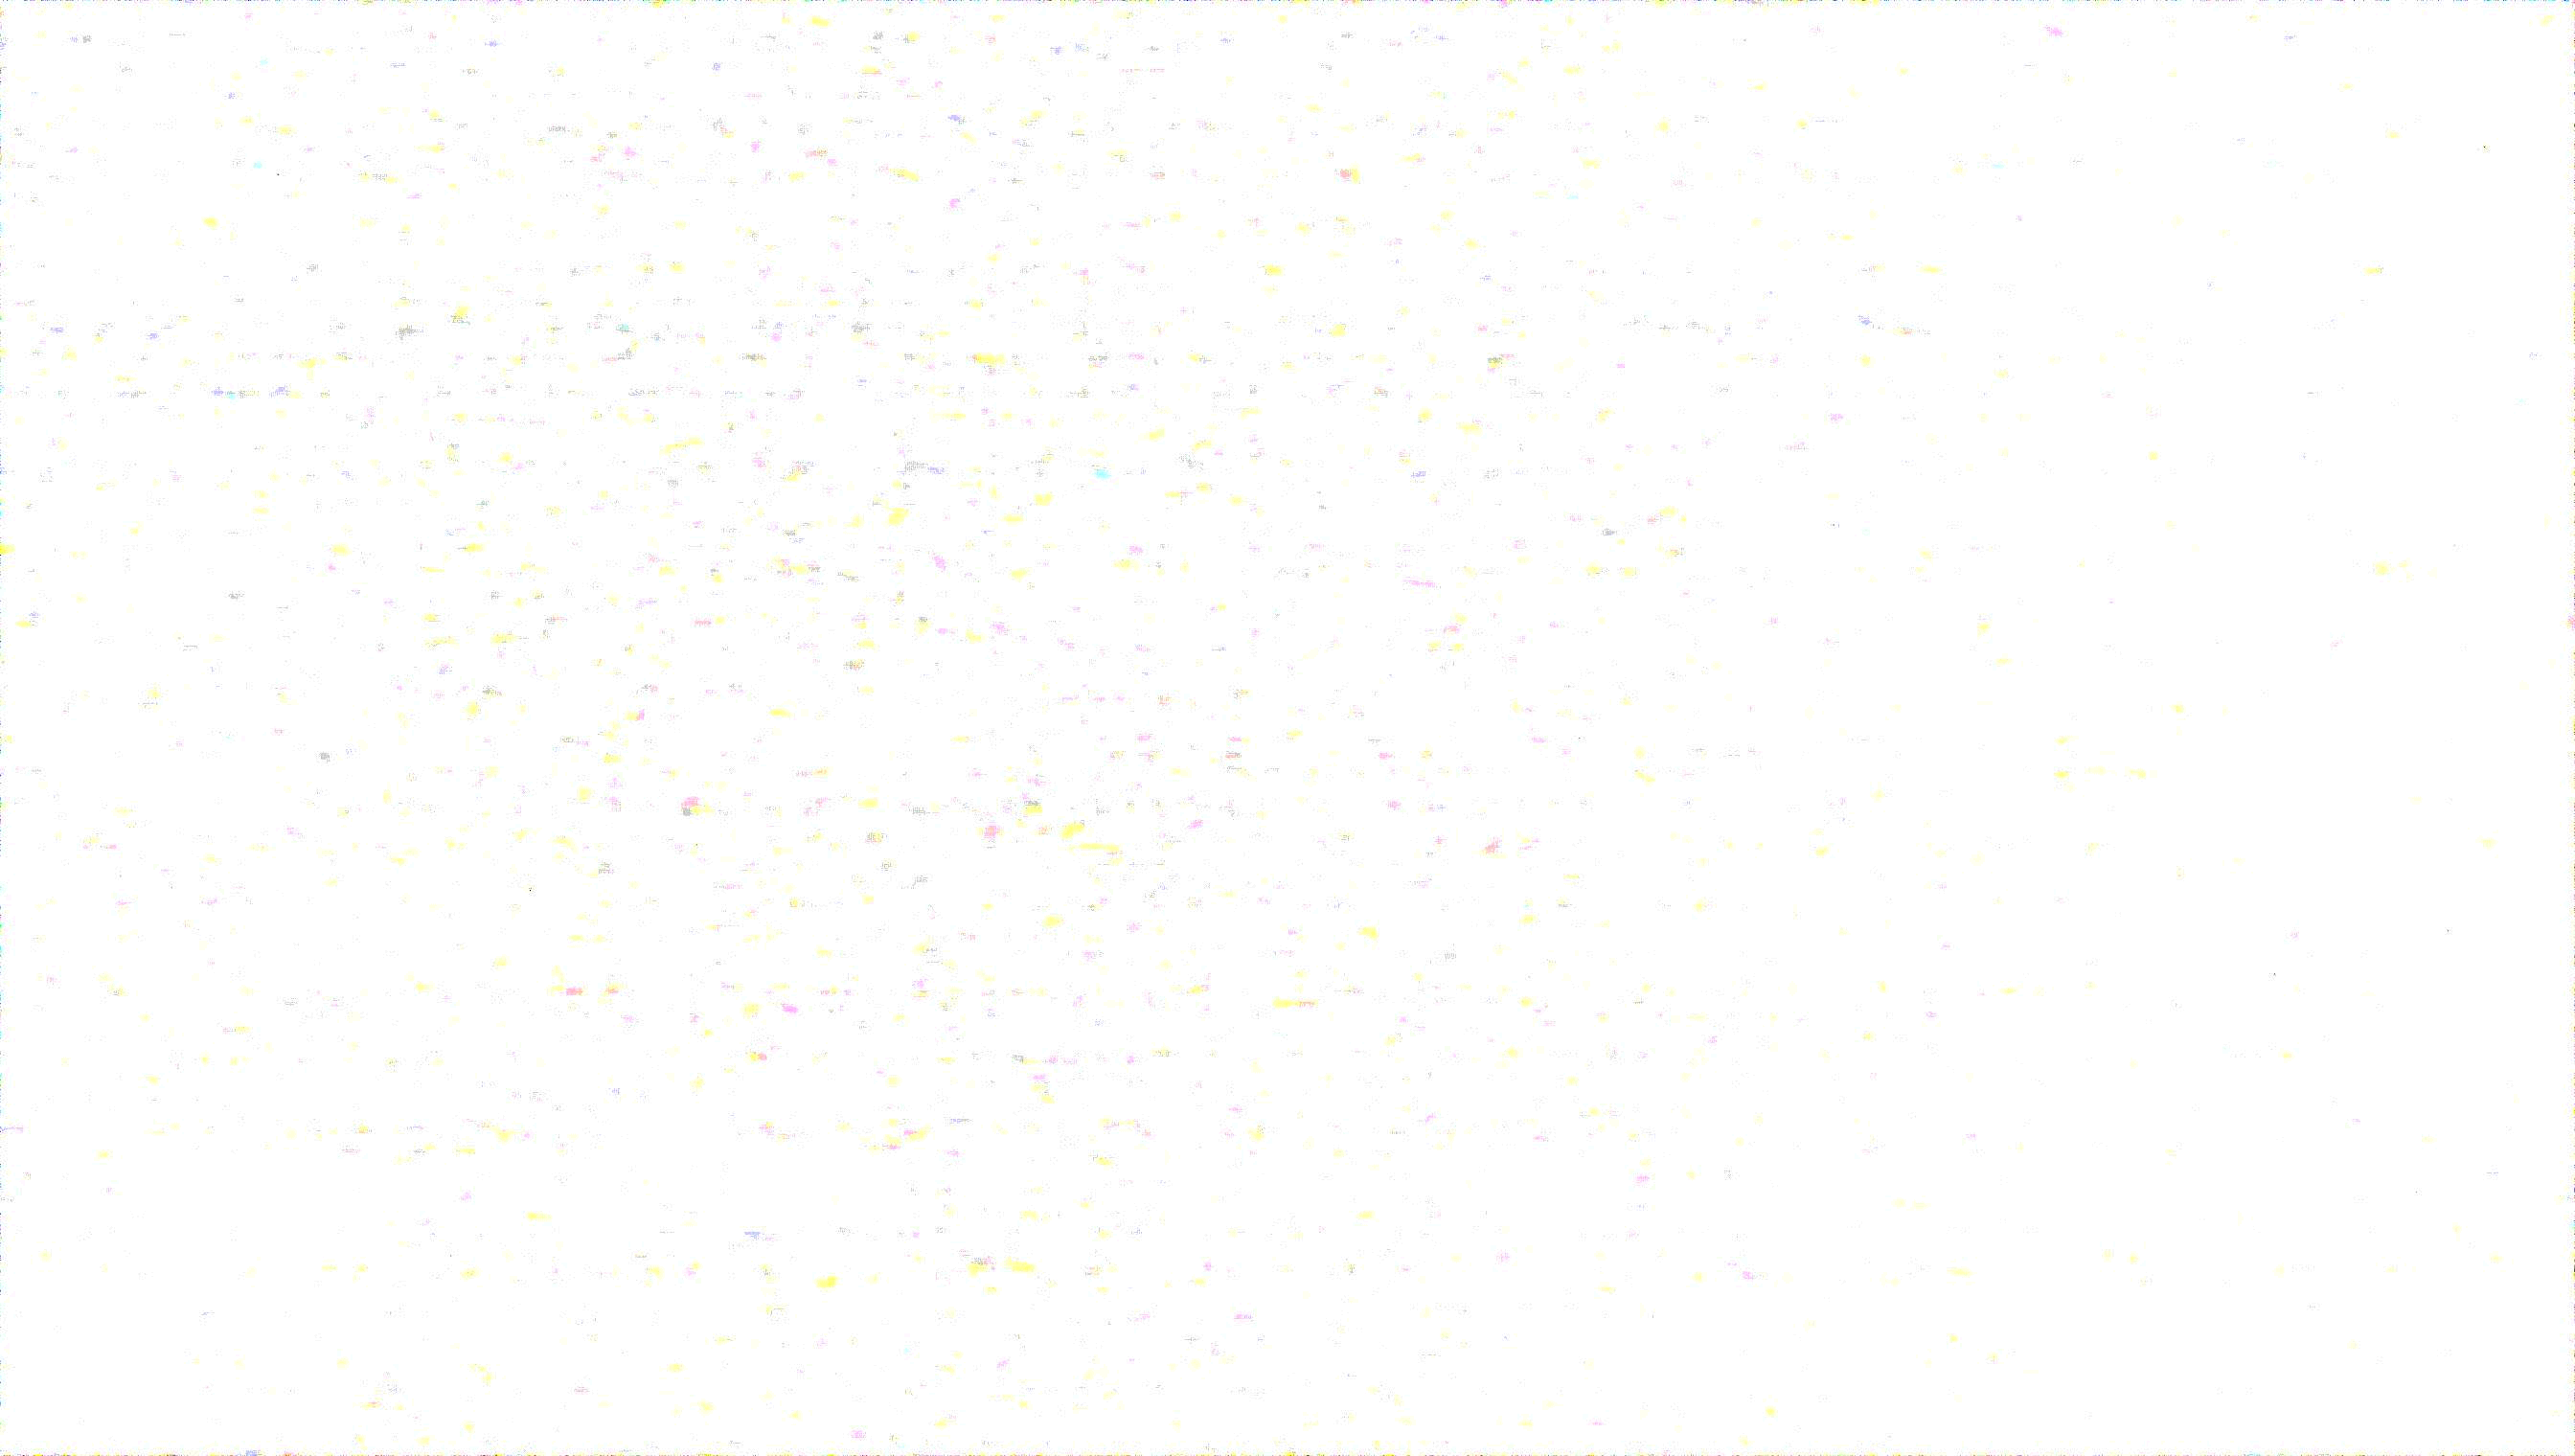
\includegraphics[width=1\linewidth]{img/NoisHight}}
	\caption{Aufnahme eines Schwarz-Bildes $(2688\times 1520)$ der Actioncam um den Faktor 7 verstärkt und invertiert.}
	\label{img_noishight}
\end{figure}

\subsection{To Do}
\begin{itemize}
	\item Patch Experts und Optimierungsfunktionen CLM
	\item Auswirkung von Pixelrauschen
	\begin{itemize}
		\item Rauschen der Actioncam bestimmen\\
		Done
		\item Simulation des Rauschens\\
		Add Gaußverteilung auf Image 
	\end{itemize}
\item Distanzen
\item Winkel
\item Auswerten der Messung
\item Wann ELSE
\item Mittlung Ergebnis / Landmarks
\item Zuverlässigkeit mit Farbkorrektur
\end{itemize}